\documentclass{bioinfo}
\copyrightyear{2008}
\pubyear{2008}
\usepackage{url}
\usepackage{verbatim}

\newif\ifnonbi
\nonbifalse
\newif\ifbi
\bitrue

\bibliographystyle{natbib}

\begin{document}
\firstpage{1}

\begin{application}

\title[Infernal 1.0]{Infernal 1.0: inference of RNA alignments}
\author[E. Nawrocki, D. Kolbe and S. Eddy]{Eric P. Nawrocki,\,$^1$ Diana L. Kolbe\,$^1$ and Sean R. Eddy\,$^1$\footnote{to whom correspondence should be addressed}}
\address{$^{1}$HHMI Janelia Farm Research Campus, Ashburn VA 20147, USA\\}

\history{Received on XXXXX; revised on XXXXX; accepted on XXXXX}

\editor{Associate Editor: XXXXXXX}

\maketitle

\begin{abstract}
\section{Summary:}
\textsc{infernal} builds consensus RNA secondary structure profiles
called covariance models (CMs), and uses them to search nucleic acid
sequence databases for homologous RNAs, or to create new sequence- and
structure-based multiple sequence alignments.

\section{Availability:}
Source code, documentation, and benchmark downloadable from
\url{http://infernal.janelia.org}. \textsc{infernal} is freely
licensed under the GNU GPLv3 and should be portable to any
POSIX-compliant operating system, including Linux and Mac OS/X.


\section{Contact:} \url{{nawrockie,kolbed,eddys}@janelia.hhmi.org}
\end{abstract}



\Easel\ is a C code library for computational analysis of biological
sequences using probabilistic models. \Easel\ is used by \HMMER\ 
\citep{hmmer,Eddy98}, the profile hidden Markov model software that
underlies the \Pfam\ protein family database
\citep{Finn06,Sonnhammer97} and several other protein family
databases. \Easel\ is also used by \Infernal\ 
\citep{infernal,NawrockiEddy07}, the covariance model software that
underlies the \Rfam\ RNA family database
\citep{Griffiths-Jones05}. 

There are other biosequence analysis libraries out there, in a variety
of languages
\citep{Vahrson96,Pitt01,Mangalam02,Butt05,Dutheil06,Giancarlo07,Doring08};
but this is ours.  \Easel\ is not meant to be comprehensive.  \Easel
is for supporting what's needed in our group's work on probabilistic
modeling of biological sequences, in applications like \HMMER\ and
\Infernal. It includes code for generative probabilistic models of
sequences, phylogenetic models of evolution, bioinformatics tools for
sequence manipulation and annotation, numerical computing, and some
basic utilities.

\Easel\ is written in ANSI/ISO C because its primary goals are high
performance and portability. Additionally, \Easel\ aims to provide an
ease of use reasonably close to Perl or Python code.

\Easel\ is designed to be reused, but not only as a black box. I might
use a black box library for routine functions that are tangential to
my research, but for anything research-critical, I want to understand
and control the source code.  It's rational to treat reusing other
people's code like using their toothbrush, because god only knows what
they've done to it. For me, code reuse more often means acting like a
magpie, studying and stealing shiny bits of other people's source
code, and weaving them into one's own nest. \Easel\ is designed so you
can easily pull useful baubles from it.

\Easel\ is also designed to enable us to publish reproducible and
extensible research results as supplementary material for our research
papers. We put work into documenting \Easel\ as carefully as any other
research data we distribute.

These considerations are reflected in \Easel design decisions.
\Easel's documentation includes tutorial examples to make it easy to
understand and get started using any given \Easel\ module, independent
of other parts of \Easel.  \Easel\ is modular, in a way that should
enable you to extract individual files or functions for use in your
own code, with minimum disentanglement work. \Easel\ uses some
precepts of object-oriented design, but its objects are just C
structures with visible, documented contents. \Easel's source code is
consciously designed to be read as a reference work. It reflects, in a
modest way, principles of ``literate programming'' espoused by Donald
Knuth. \Easel\ code and documentation are interwoven. Most of this
book is automatically generated from \Easel's source code.



\section{Quick start}

Let's start with a quick tour. If you have any experience with the
variable quality of bioinformatics software, the first thing you want
to know is you can get Easel compiled -- without having to install a
million dependencies first. The next thing you'll want to know is
whether \Easel\ is going to be useful to you or not. We'll start with
compiling it. You can compile \Easel\ and try it out without
permanently installing it.



\subsection{Downloading and compiling Easel for the first time}

Easel is self-sufficient, with no dependencies other than what's
already on your system, provided you have an ANSI C99 compiler
installed.  You can obtain an \Easel\ source tarball and compile it
cleanly on any UNIX, Linux, or Mac OS/X operating system with an
incantation like the following (where \ccode{xxx} will be the current
version number):

\begin{cchunk}
% wget http://eddylab.org/easel/easel.tar.gz
% tar zxf easel.tar.gz
% cd easel-xxx
% ./configure
% make
% make check
\end{cchunk}

The \ccode{make check} command is optional. It runs a battery of
quality control tests. All of these should pass. You should now see
\ccode{libeasel.a} in the directory. If you look in the directory
\ccode{miniapps}, you'll also see a bunch of small utility programs,
the \Easel\ ``miniapps''.

There are more complicated things you can do to customize the
\ccode{./configure} step for your needs. That includes customizing the
installation locations. If you decide you want to install
\Easel\ permanently, see the full installation instructions in
chapter~\ref{chapter:installation}.



\subsection{Cribbing from code examples}

Every source code module (that is, each \ccode{.c} file) ends with one
or more \esldef{driver programs}, including programs for unit tests
and benchmarks. These are \ccode{main()} functions that can be
conditionally included when the module is compiled. The very end of
each module is always at least one \esldef{example driver} that shows
you how to use the module. You can find the example code in a module
\eslmod{foo} by searching the \ccode{esl\_foo.c} file for the tag
\ccode{eslFOO\_EXAMPLE}, or just navigating to the end of the file. To
compile the example for module \eslmod{foo} as a working program, do:

\begin{cchunk}
   % cc -o example -L. -I. -DeslFOO_EXAMPLE esl_foo.c -leasel -lm
\end{cchunk}

You may need to replace the standard C compiler \ccode{cc} with a
different compiler name, depending on your system. Linking to the
standard math library (\ccode{-lm}) may not be necessary, depending on
what module you're compiling, but it won't hurt. Replace \ccode{foo}
with the name of a module you want to play with, and you can compile
any of Easel's example drivers this way.

To run it, read the source code (or the corresponding section in this
book) to see if it needs any command line arguments, like the name of
a file to open, then:

\begin{cchunk}
   % ./example <any args needed>
\end{cchunk}

You can edit the example driver to play around with it, if you like,
but it's better to make a copy of it in your own file (say,
\ccode{foo\_example.c}) so you're not changing \Easel's code. When you
extract the code into a file, copy what's between the \ccode{\#ifdef
eslFOO\_EXAMPLE} and \ccode{\#endif /*eslFOO\_EXAMPLE*/} flags that
conditionally include the example driver (don't copy the flags
themselves). Then compile your example code and link to \Easel\ like
this:

\begin{cchunk}
   % cc -o foo_example -L. -I. foo_example.c -leasel -lm
\end{cchunk}

\subsection{Cribbing from Easel miniapplications}

The \ccode{miniapps} directory contains \Easel's
\esldef{miniapplications}: several utility programs that \Easel\
installs, in addition to the library \ccode{libeasel.a} and its header
files.

The miniapplications are described in more detail later, but for the
purpose of getting used to how \Easel\ is used, they provide you some
more useful examples of small \Easel-based applications that are a
little more complicated than individual module example drivers.

You can probably get a long way into \Easel\ just by browsing the
source code of the modules' examples and the miniapplications. If
you're the type (like me) that prefers to learn by example, you're
done, you can close this book now. 



\section{Overview of Easel's modules}

Possibly your next question is, does \Easel\ provide any functionality
you're interested in?

Each \ccode{.c} file in \Easel\ corresponds to one \Easel\
\esldef{module}.  A module consists of a group of functions for some
task. For example, the \eslmod{sqio} module can automatically parse
many common unaligned sequence formats, and the \eslmod{msa} module
can parse many common multiple alignment formats.

There are modules concerned with manipulating biological sequences and
sequence files (including a full-fledged parser for Stockholm multiple
alignment format and all its complex and powerful annotation markup):

\begin{center}
\begin{tabular}{p{1in}p{3.7in}}
\eslmod{sq}       & Single biological sequences            \\
\eslmod{msa}      & Multiple sequence alignments and i/o   \\
\eslmod{alphabet} & Digitized biosequence alphabets        \\
\eslmod{randomseq}& Sampling random sequences              \\
\eslmod{sqio}     & Sequence file i/o                      \\
\eslmod{ssi}      & Indexing large sequence files for rapid random access \\
\end{tabular}
\end{center}

There are modules implementing common operations on multiple sequence
alignments (including many published sequence weighting algorithms,
and a memory-efficient single linkage sequence clustering algorithm):

\begin{center}
\begin{tabular}{p{1in}p{3.7in}}
\eslmod{msacluster} & Efficient single linkage clustering of aligned sequences by \% identity\\
\eslmod{msaweight}  & Sequence weighting algorithms \\
\end{tabular}
\end{center}

There are modules for probabilistic modeling of sequence residue
alignment scores (including routines for solving for the implicit
probabilistic basis of arbitrary score matrices):

\begin{center}
\begin{tabular}{p{1in}p{3.7in}}
\eslmod{scorematrix} & Pairwise residue alignment scoring systems\\
\eslmod{ratematrix}  & Standard continuous-time Markov models of residue evolution\\
\eslmod{paml}        & Reading PAML data files (including rate matrices)\\
\end{tabular}
\end{center}

There is a module for sequence annotation:

\begin{center}
\begin{tabular}{p{1in}p{3.7in}}
\eslmod{wuss} & ASCII RNA secondary structure annotation strings\\
\end{tabular}
\end{center}

There are modules implementing some standard scientific numerical
computing concepts (including a free, fast implementation of conjugate
gradient optimization):

\begin{center}
\begin{tabular}{p{1in}p{3.7in}}
\eslmod{vectorops} & Vector operations\\
\eslmod{dmatrix}   & 2D matrix operations\\
\eslmod{minimizer} & Numerical optimization by conjugate gradient descent\\
\eslmod{rootfinder}& One-dimensional root finding (Newton/Raphson)\\
\end{tabular}
\end{center}

There are modules implementing phylogenetic trees and evolutionary
distance calculations:

\begin{center}
\begin{tabular}{p{1in}p{3.7in}}
\eslmod{tree}     & Manipulating phylogenetic trees\\
\eslmod{distance} & Pairwise evolutionary sequence distance calculations\\
\end{tabular}
\end{center}

There are a number of modules that implement routines for many common
probability distributions (including maximum likelihood fitting
routines):

\begin{center}
\begin{tabular}{p{1in}p{3.7in}}
\eslmod{stats}       & Basic routines and special statistics functions\\
\eslmod{histogram}   & Collecting and displaying histograms\\
\eslmod{dirichlet}   & Beta, Gamma, and Dirichlet distributions\\
\eslmod{exponential} & Exponential distributions\\
\eslmod{gamma}       & Gamma distributions\\
\eslmod{gev}         & Generalized extreme value distributions\\
\eslmod{gumbel}      & Gumbel (Type I extreme value) distributions\\
\eslmod{hyperexp}    & Hyperexponential distributions\\
\eslmod{mixdchlet}   & Mixture Dirichlet distributions and priors\\
\eslmod{mixgev}      & Mixture generalized extreme value distributions\\
\eslmod{normal}      & Normal (Gaussian) distributions\\
\eslmod{stretchexp}  & Stretched exponential distributions\\
\eslmod{weibull}     & Weibull distributions\\
\end{tabular}
\end{center}

There are several modules implementing some common utilities
(including a good portable random number generator and a powerful
command line parser):

\begin{center}
\begin{tabular}{p{1in}p{3.7in}}
\eslmod{cluster}    & Efficient single linkage clustering\\
\eslmod{fileparser} & Parsing simple token-based (tab/space-delimited) files\\
\eslmod{getopts}    & Parsing command line arguments and options.\\
\eslmod{keyhash}    & Hash tables for emulating Perl associative arrays\\
\eslmod{random}     & Pseudorandom number generation and sampling\\
\eslmod{regexp}     & Regular expression matching\\
\eslmod{stack}      & Pushdown stacks for integers, chars, pointers\\
\eslmod{stopwatch}  & Timing parts of programs\\
\end{tabular}
\end{center}

There are some specialized modules in support of accelerated and/or parallel computing:

\begin{center}
\begin{tabular}{p{1in}p{3.7in}}
\eslmod{sse}     & Routines for SSE (Streaming SIMD Intrinsics) vector computation support on Intel/AMD platforms\\
\eslmod{vmx}     & Routines for Altivec/VMX vector computation support on PowerPC platforms\\
\eslmod{mpi}     & Routines for MPI (message passing interface) support\\
\end{tabular}
\end{center}

\section{Navigating documentation and source code}

The quickest way to learn about what each module provides is to go to
the corresponding chapter in this document. Each chapter starts with a
brief introduction of what the module does, and highlights anything
that \Easel's implementation does that we think is particularly
useful, unique, or powerful. That's followed by a table describing
each function provided by the module, and at least one example code
listing of how the module can be used. The chapter might then go into
more detail about the module's functionality, though many chapters do
not, because the functionality is straightforward or self-explanatory.
Finally, each chapter ends with detailed documentation on each
function.

\Easel's source code is designed to be read. Indeed, most of this
documentation is generated automatically from the source code itself
-- in particular, the table listing the available functions, the
example code snippets, and the documentation of the individual
functions.

Each module \ccode{.c} file starts with a table of contents to help
you navigate.\footnote{\Easel\ source files are designed as complete
free-standing documents, so they tend to be larger than most people's
\ccode{.c} files; the more usual practice in C programming is to have
a smaller number of functions per file.} The first section will often
define how to create one or more \esldef{objects} (C structures) that
the module uses. The next section will typically define the rest of
the module's exposed API. Following that are any private (internal)
functions used in the module. Last are the drivers, including
benchmarks, unit tests, and one or more examples.

Each function has a structured comment header that describes how it is
called and used, including what arguments it takes, what it returns,
and what error conditions it may raise. These structured comments are
extracted for inclusion in this document, so what you read here for
each function's documentation is identical to what is in the source
code.




\section{Usage} 

A CM is built from a Stockholm format multiple sequence alignment (or
single RNA sequence) with consensus secondary structure annotation
marking which positions of the alignment are single stranded and which
are base paired \citep{infguide03}. CMs assign position specific
scores for the four possible residues at single stranded positions,
the sixteen possible base pairs at paired positions, and for
insertions and deletions. These scores are log-odds scores derived
from the observed counts of residues, base pairs, insertions and
deletions in the input alignment, combined with prior information
derived from structural ribosomal RNA alignments.  CM parameterization
has been described in more detail elsewhere
\citep{Eddy94,Eddy02b,KleinEddy03,infguide03,NawrockiEddy07}.

\textsc{infernal} is composed of several programs that are used in
combination by following four basic steps: 

\begin{enumerate}
\item Build a CM from a structural alignment with \emph{cmbuild}.
\item Calibrate a CM for homology search with \emph{cmcalibrate}.
\item Search databases for putative homologs with \emph{cmsearch}.
\item Align putative homologs to a CM with \emph{cmalign}.
\end{enumerate}

The calibration step is optional and computationally expensive (4
hours on a 3.0 GHz Intel Xeon for a CM of a typical RNA family of
length 100 nt), but is required to obtain E-values that estimate
the statistical significance of hits in a database
search. \emph{cmcalibrate} will also determine appropriate HMM filter
thresholds for accelerating searches without an appreciable loss of
sensitivity. Each model only needs to be calibrated once.



\section{Performance}

A published benchmark (independent of our lab) \citep{Freyhult07} and
our own internal benchmark used during development
\citep{NawrockiEddy07} both find that \textsc{infernal} and other CM
based methods are the most sensitive and specific tools for structural
RNA homology search among those tested. Figure~1 shows updated results
of our internal benchmark comparing \textsc{infernal} 1.0 to the
previous version (0.72) that was benchmarked in \citet{Freyhult07},
and also to family-pairwise-search with BLASTN \citep{Altschul97,
Grundy98b}.  \textsc{infernal}'s sensitivity and specificity have
greatly improved, due mainly to three relevant improvements in the
implementation \citep{infguide03}: a biased composition correction to
the raw log-odds scores, the use of Inside log likelihood scores (the
summed score of all possible alignments of the target sequence) in
place of CYK scores (the single maximum likelihood alignment score),
and the introduction of approximate E-value estimates for the scores.

The benchmark dataset used in Figure~1 includes query alignments and
test sequences from 51 \textsc{Rfam} (release 7) families (details in
\citep{NawrockiEddy07}).  No query sequence is more than 60\% identical
to a test sequence.  The 450 total test sequences were embedded at
random positions in a 10 Mb ``pseudogenome''.  Previously we generated
the pseudogenome sequence from a uniform residue frequency
distribution \citep{NawrockiEddy07}.  Because base composition biases
in the target sequence database cause the most serious problems in
separating significant CM hits from noise, we improved the realism of
the benchmark by generating the pseudogenome sequence from a 15-state
fully connected first-order hidden Markov model (HMM) trained by
Baum-Welch expectation maximization \citep{Durbin98} on genome
sequence data from a wide variety of species.  Each of the 51 query
alignments was used to build a CM and search the pseudogenome, a
single list of all hits for all families were collected and ranked,
and true and false hits were defined (as described in
\citet{NawrockiEddy07}), producing the ROC curves in Figure~1.

\textsc{infernal} searches require a large amount of compute time (our
10 Mb benchmark search takes about 30 hours per model on average
(Figure~1)). To alleviate this, \textsc{infernal} 1.0 implements two
rounds of filtering.  When appropriate, the HMM filtering technique
described by \citet{WeinbergRuzzo06} is applied first with filter
thresholds configured by \emph{cmcalibrate} (occasionally a model with
little primary sequence conservation cannot be usefully accelerated by
a primary sequence-based filter as explained in \citep{infguide03}).  The
query-dependent banded (QDB) CYK maximum likelihood search algorithm
is used as a second filter with relatively tight bands ($\beta$=
$10^{-7}$, the $\beta$ parameter is the subtree length probability
mass excluded by imposing the bands as explained in
\citep{NawrockiEddy07}).  Any sequence fragments that survive the
filters are searched a final time with the Inside algorithm (again
using QDB, but with looser bands ($\beta$= $10^{-15}$)).  In our
benchmark, the default filters accelerate similarity search by about
30-fold overall, while sacrificing a small amount of sensitivity
(Figure~1). This makes version 1.0 substantially faster than
0.72. \textsc{BLAST} is still orders of magnitude faster, but
significantly less sensitive than \textsc{infernal}. Further
acceleration remains a major goal of \textsc{infernal} development.

The computational cost of CM alignment with \emph{cmalign} has been a
limitation of previous versions of \textsc{infernal}. Version 1.0 now
uses a constrained dynamic programming approach first developed by
\citet{Brown00} that uses sequence-specific bands derived from a
first-pass HMM alignment. This technique offers a dramatic speedup
relative to unconstrained alignment, especially for large RNAs such as
small and large subunit (SSU and LSU) ribosomal RNAs, which can now be
aligned in roughly 1 and 3 seconds per sequence, respectively, as
opposed to 12 minutes and 3 hours in previous versions.  This
acceleration has facilitated the adoption of \textsc{infernal} by RDP,
one of the main ribosomal RNA databases \citep{Cole09}.



\section{Discussion}

FST is a general method for determining filter survival score
thresholds to achieve a target level of sensitivity that can be
applied to any database similarity search method.  It is particularly
easy to apply FST to search methods that use generative probabilistic
models because the requisite test sequences for the threshold
calibration can be sampled directly from the model. Here, we have
explored the performance of FST on RNA similarity searches with CMs
using this sampling technique, and show that on our benchmark, using
HMM filters with FST calibrated thresholds reduces running time by
25-fold with a modest cost to sensitivity.
%By combining the HMM
%filters with a second round of filter using the banded CYK CM search
%algorithm the running time decreases another three-fold without an
%appreciable loss in sensitivity, resulting in a net speedup of about
%100-fold relative to non-filtered searches.

\begin{comment}
The slow speed of CM searches been the most serious obstacle to the
use of the \textsc{infernal} software for annotating RNAs in databases
and genomes. Without using filters, running the most sensitive CM
search algorithm with \textsc{infernal} version 1.0 required about
1700 hours to complete our benchmark search of 51 families against
both strands of a 10 Mb database. We have shown that by combining FST
calibrated HMM filters and QDB CYK filters with $F$ and $\beta$
parameters that do not significantly compromise specificity or
sensitivity, the running time drops about 100-fold to about 16 hours.
%Eventually, we want to be able to use \textsc{infernal} to
%annotate RNAs in large genomes in at most a few days. To run the 1371
%\textsc{Rfam} release 9.1 families against the entire human genome
%would require about 15 CPU years (down from 800 CPU years with
%\textsc{infernal} 0.72).
\end{comment}

FST calibrated thresholds are query-dependent, and are most
advantageous relative to query-independent thresholds, such as the
target $S$ thresholding method, for filtering methods in which
different queries require significantly different surivival thresholds
to achieve high sensitivity. We expect this is mostly true for
filtering methods that score sequences in a qualitatively different
way than the final search method, as in the case reported here which
uses HMMs to filter, that score only primary sequence conservation,
for CMs, which score both primary sequence and secondary structure
conservation. However, when the filter scoring metric is more closely
related to the final metric, simpler thresholding strategies,
such as picking a single query independent threshold that empirically
performs well on a benchmark may be more reasonable. This is the case
with our experiments using the CM CYK algorithm as a filter for the CM
Inside algorithm.

FST calibrated thresholds are also dependent on the reporting
threshold of the final search method. This is demonstrated for CM
filtering by the trajectory of the large, open circle points in
Figure~\ref{Fig:fst} that indicate filter threshold/final threshold
pairs $(T,C)$ pairs. As the CM reporting score threshold increases
from $a$ to $b$, the filter survival threshold necessary to maintain
sensitivity also increases because the filter can now afford to miss
hits in the score range $a$ to $b$ without affecting sensitivity.  And
as this survival threshold increases, so does the acceleration gained
from the filter.  This feature of FST is useful for search methods
where the reporting threshold chosen by users can vary widely for
different applications.  This is the case with CMs, where searches can
range in magnitude from \textsc{Rfam}'s annotation of
the 120 Gb RFAMSEQ database, to searches in a prokaryotic genome of a
few Mb. A reporting threshold of $E=1$ in these two types of searches
corresponds to significantly different bit scores because of the large
size difference of the databases being searched, thus the survival
reporting threshold will differ markedly between them, offering
greater acceleration for the large RFAMSEQ search than for the
prokaryotic genome search.

%By combining the HMM
%filters with a second round of filter using the banded CYK CM search
%algorithm the running time decreases another three-fold without an
%appreciable loss in sensitivity, resulting in a net speedup of about
%100-fold relative to non-filtered searches.

The slow speed of CM searches has been the most serious obstacle to
the use of \textsc{infernal} for annotating RNAs in databases and
genomes. Without using filters, running the most sensitive CM search
algorithm with \textsc{infernal} version 1.01 required about 1500
hours to complete our benchmark search of 51 families against both
strands of a 10 Mb database. We have shown that by combining FST
calibrated HMM filters and QDB CYK filters with $F$, $S_{min}$, and
$\beta$ parameters that do not significantly compromise specificity or
sensitivity, the running time drops 70-fold to about 20 hours.
Eventually, we want to be able to use \textsc{infernal} to annotate
RNAs in large genomes in at most a few days. If our benchmark results
hold for the general case, to run the 1371 \textsc{Rfam} release 9.1
families against the entire human genome would require about 20 CPU
years (compared to 1500 CPU years for a non-filtered search), which
means further acceleration remains an important goal of
\textsc{infernal} development.

We can imagine several ways to make \textsc{infernal} faster. One is
to use faster filters. A new version (3.0) of the \textsc{HMMER}
software package is in it's last throes of development, and includes
significantly faster HMM search algorithm implementations than those
in \textsc{infernal} 1.01. We plan to incorporate those
implementations within \textsc{infernal} for filtering.  Other
possible filtering strategies include using BLAST-like
algorithms, or keyword based methods such as those described by
\citet{ZhangBafna06}. But the HMM filters are not the rate limiting
step in CM searches, the time required to run the filter on our
benchmark is about one third the total time of the search
(Table~\ref{Tab:merlist} rows 18 and 19).  So, unless we can design filters
with lower survival fractions, the maximum acceleration we can gain
from faster filters is about 33\%.  A complementary approach is to
write faster implementations of the final CM search algorithms, Inside
and CYK.  Ongoing work on \textsc{HMMER} 3 has suggested that
optimizing the dynamic programming search algorithm implementations
using single-instruction multiple data (SIMD) paralellism could yield
significant speedups.
%Speed can be addressed at the hardware level as
%well, (MORE HERE FROM SEAN). 
Developing these improvements -- and incorporating
them into a widely useful, freely available codebase -- are priorities
for us.


\begin{comment}
The slow speed of CM searches been the most serious obstacle to the
use of the \textsc{infernal} software for annotating RNAs in databases
and genomes. Without using filters, running the most sensitive CM
search algorithm with \textsc{infernal} version 1.01 required about
1700 hours to complete our benchmark search of 51 families against
both strands of a 10 Mb database. We have shown that by combining FST
calibrated HMM filters and QDB CYK filters with $F$ and $\beta$
parameters that do not significantly compromise specificity or
sensitivity, the running time drops about 100-fold to about 16
hours. Eventually, we want to be able to use \textsc{infernal} to
annotate RNAs in large genomes in at most a few days. To run the 1371
\textsc{Rfam} release 9.1 families against the entire human genome
would require about 15 CPU years (down from 800 CPU years with
\textsc{infernal} 0.72).
%1371 ~= 51 * 28; 
%3Gb  ~= 10Mb * 300;
%28 * 300 ~= 8500
%8500 * 16  =~ 136,000
%365 * 24 = 8,760 hours in a year
%136,000 / 8,760 =~ 15 years
%8500 * 800 =~ 6,800,000 
%6,800,000 / 8,760 = 776 years
%
\end{comment}




\section*{Acknowledgement}

We thank Goran Ceric for his peerless skill in managing Janelia Farm's
high performance computing resources.

\paragraph*{Funding\textcolon} 
\textsc{Infernal} development is supported by the Howard Hughes
Medical Institute. It has been supported in the past by an NIH NHGRI
training grant (T32-HG000045) to EPN, an NSF Graduate Fellowship to
DLK, NIH R01-HG01363, and a generous endowment from Alvin Goldfarb.


\begin{figure}[h]
\centerline{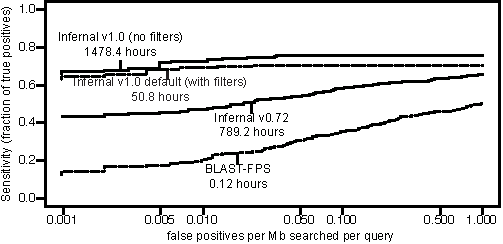
\includegraphics{figs/roc-short}}
\caption{\textbf{ROC curves for the benchmark.}  Plots are shown for
the new \textsc{infernal} 1.0 with and without filters, for the old
\textsc{infernal} 0.72, and for family-pairwise-searches (FPS) with
\textsc{blastn}. CPU times are total times for all 51 family
searches measured for single execution threads on 3.0 GHz Intel Xeon
 processors. The \textsc{infernal} 1.0 times do not include time
 required for model calibration.}


\label{Fig:01}
\end{figure}

%%%%%%%%%%%%%%%%%%%%%%%%%%%%%%%%%%%%%%%%%%%%%%%%%%%%%%%%%%%%%%%%%%%%%%%%%%%%%%%%%%%%%
%
%     please remove the " % " symbol from \centerline{\includegraphics{fig01.eps}}
%     as it may ignore the figures.
%
%%%%%%%%%%%%%%%%%%%%%%%%%%%%%%%%%%%%%%%%%%%%%%%%%%%%%%%%%%%%%%%%%%%%%%%%%%%%%%%%%%%%%%

%\bibliographystyle{bioinformatics}
\bibliography{master,books,lab,new}

\end{application}
\end{document}

% Table below was removed to meet the 2 page limit
\begin{comment}
\begin{table}[!t]
\processtable{
\textbf{Calibration, search, and alignment running times for seven known
    structural RNAs of various sizes.} 
    \label{Tab:01}}
%\ifnonbi \caption{ \fi
\textbf{Table 1: Calibration, search, and alignment running times for seven known
    structural RNAs of various sizes.} CPU times are measured on
    3.0 GHz Intel Xeon processors with 8 GB RAM, running Red Hat AS4
    Linux operating systems. All times were single execution threads
    except for SSU and LSU calibrations and searches
    which were run in parallel using MPI (OpenMPI) on 12 CPUs (times
    reported are actual times multiplied by 12).  ``Length'' is the
    number of consensus positions (positions that contain gaps in
    fewer than 50\% of the aligned sequences) in the input alignment.
    Randomly generated sequence of length 20 Mb (for filtered) and 2
    Mb (for non-filtered) was used for the searches. Query alignments
    are all Rfam 9.0 seed alignments (RF00005, RF00001, RF00168, RF00017,
    RF00011) \citep{Gardner09} except for SSU and LSU rRNA which were
    subsets of alignments at the Comparative RNA Website \citep{Cannone02}.
%(\textbf{*}) Faster non-CM methods, such as Blast or
%    HMMs, are recommended for finding SSU and LSU rRNA sequences due
%    to the high level of primary sequence conservation in those
%    families.
\ifnonbi } \fi

{%%%%%%%%%%%%%%%%%%%%%%%%%%%%%%%%%%%%%%%%%%%%%%%%%%%%%%%%%%%%%%%%%%%%%%%
% The 7 RNAs table, running times for various applications for 
% 7 RNAs

% Table without average percent id in training alignment
\begin{tabular}{lrr|rr|r}\ifbi \toprule \fi
       &           & calibration  & \multicolumn{2}{c|}{search (min/Mb)} & alignment \\
family & length    & (hours)      & no filters& w/filters                & (sec/seq) \\\ifbi \midrule \fi \ifnonbi \hline \fi
tRNA    & 71       &       3.2h   &     23.5m &        4.4m&  0.01s \\
5S rRNA & 119      &       4.4h   &     29.3m &        1.1m&  0.03s \\
Lysine riboswitch & 183 &  8.9h   &    100.5m &        1.3m&  0.06s \\
%riboswitch &       &              &           &           &        \\
SRP RNA & 304      &      13.5h   &    166.0m &        3.0m&  0.18s \\
RNaseP  & 365      &      16.8h   &    205.6m &        0.9m&  0.19s \\
SSU rRNA& 1466     &      84.5h   &   1265.5m &       17.6m&  1.10s \\
LSU rRNA& 2909     &     169.7h   &   3907.6m &      740.4m&  3.34s \\ \ifbi \botrule \fi
\end{tabular}


% Table with average percent id in training alignment
%\begin{tabular}{lrrr|rr|r}\ifbi \toprule \fi
%       &           & avg \% id& calib-       & \multicolumn{2}{c|}{search}          &           \\
%       &           & in train-& ration       & \multicolumn{2}{c|}{(min/Mb)}        & alignment \\
%family & length    & ing aln  & (hours)      & no filters& w/filters                & (sec/seq) \\\ifbi \midrule \fi \ifnonbi \hline \fi
%tRNA    & 71       & 44\%     
%5S rRNA & 119      & 56\%     
%SRP RNA & 304      & 46\%     
%RNaseP  & 365      & 65\%     
%SSU rRNA& 1545     & 77\%     
%LSU rRNA& 2898     & 82\%     
%\end{tabular}


%
% alignment times (a subset of these will be in final table)
% 
% Timings from ~/notebook/8_0909_manuscript_inf-1_appnote/00LOG
% 
% family          & non-banded CYK & HMM banded CYK & HMM banded optacc (default)
%
% tRNA            &       0.049    &         0.0045 &            0.0129
% 5S rRNA         &       0.2023   &         0.0095 &            0.0256
% SRP RNA         &       5.4509   &         0.0615 &            0.1680
% RNase P         &      11.958    &         0.0721 &            0.1759
% SSU rRNA        &     724.201    &         0.7691 &            1.0870
% LSU rRNA        &   11819.9      &         2.5347 &            3.1206
%
}{CPU times are measured on 3.0 GHz Intel Xeon
processors with 8 GB RAM, running Red Hat AS4 Linux operating
systems. All times were single execution threads except for SSU and
LSU calibrations and searches which were run in parallel using MPI
(OpenMPI) on 12 CPUs (times reported are actual times multiplied by
12).  ``Length'' is the number of consensus positions (positions that
contain gaps in fewer than 50\% of the aligned sequences) in the input
alignment.  Randomly generated sequence of length 20 Mb (for filtered)
and 2 Mb (for non-filtered) was used for the searches. Alignment files
\citep{Gardner09,Cannone02}, CM files and instructions for reproduction
are in the supplementary material.}
\end{table}
\end{comment}
